\documentclass{article}
\usepackage{neurips}
\usepackage{booktabs}
\usepackage{multirow}

\title{Semantic Discovery Is Not Enough:\\
Complementarity Gaps and Capability Spam in Open Agent Networks}

\author{
  Anonymous Author(s)\\
  Affiliation withheld for double blind review\\
  \texttt{anonymous@domain.com}
}

\begin{document}
\maketitle

\begin{abstract}
Open agent networks need more than a good match to a single agent card.
Many jobs require a small team whose skills cover a multi part requirement, and the agents advertising those skills may not be honest.
We study this setting as a network problem rather than a single agent demo.
First we show, with short existence arguments, that cosine style ranking can miss complementary specialists even when advertisements are truthful, and that overclaiming can break any selector that trusts ads as ground truth.
Then we introduce AgenticWeb Micro, a controllable open registry benchmark with honest ads, capability spam, and churn.
We compare random selection, cosine retrieval, greedy skill cover, Claude Sonnet~5 reading natural language marketplace cards, and a cover method that adds sandbox probes plus reputation.
On honest ads, cover based selection reaches perfect team success while similarity and Claude sit slightly lower.
Under spam, advertisement trusting cover collapses to zero, Claude tracks the similarity drop, and the probe aware method recovers near perfect success.
Offline ablations show the same pattern across spam rates and registry sizes, and that either probes or outcome reputation can restore cover if given a few epochs.
The practical point is narrow and, we think, timely for the Agentic Web: semantic discovery helps, but team routing on open networks also needs coverage objectives and outcome grounded trust.
\end{abstract}

\section{Introduction}

Most agent demos still look like one model calling one tool.
The Agentic Web is a different object~\citep{projectnanda2026,raskar2025}.
Agents come and go, advertise themselves in public cards, and get hired into short lived teams.
If a user goal needs web search, SQL, and summarization at once, someone has to assemble a team that actually covers those needs.

The industry default is semantic discovery.
Cards are embedded, or an LLM reads the text and ranks candidates~\citep{karpukhin2020,lewis2020}.
That is a sensible first step for single agent lookup.
It is a weaker fit for team formation.
Similarity rewards agents that look like the whole job.
A set of specialists can look worse one by one, even when they are the only way to cover the requirement together.

Open networks add a second problem that closed demos often hide.
Agents can overclaim.
A listing can sound broader than the underlying tools.
Any router that treats advertisements as facts will then hire spam.

We treat the registry and the team as the unit of analysis, in line with the workshop framing~\citep{projectnanda2026}.
The paper makes three concrete contributions:
\begin{enumerate}
    \item A small formal model of open registry team formation, with two existence results on complementarity gaps and capability spam.
    \item AgenticWeb Micro, a reproducible micro benchmark with honest, spam, and churn plus spam regimes, including natural language cards and a Claude Sonnet~5 router.
    \item Main results plus ablations showing when similarity and LLM ranking fail, when blind cover fails harder, and when probes plus reputation put success back.
\end{enumerate}

We are not proposing a new web protocol.
We are trying to make the discovery failure modes hard to ignore, with numbers and a public artifact.

\section{Related work}

\paragraph{Multi agent systems and LLM agents.}
Classical multi agent work studied cooperation, negotiation, and learning in groups~\citep{wooldridge2009,stone2000}.
Recent LLM agents wrap tools and talk to each other inside orchestrated graphs~\citep{shen2023,wu2023,yao2023,schick2023}.
Most of that stack still assumes a designer chose the cast, or that tools are locally trusted.
We instead start from an open registry where membership is not under one owner's control.

\paragraph{Retrieval and semantic matching.}
Dense retrieval and RAG popularized embedding based selection over large corpora~\citep{karpukhin2020,lewis2020}.
Agent directories copy the same idea onto skill cards.
Our honest regime shows why that transfer is incomplete for teams: high similarity to the query is not the same as joint cover.
Our spam regime shows a second break: free text cards are easy to inflate.

\paragraph{Trust, reputation, and the Agentic Web.}
Work on machine behaviour and population scale AI already warned that interaction patterns matter as much as model scores~\citep{rahwan2019}.
NANDA style indexes and trust fabric proposals push naming, discovery, and economic coordination for internet scale agents~\citep{raskar2025,balija2025}.
We sit next to that line, but on the learning and evaluation side the workshop asks for~\citep{projectnanda2026}: what fails when discovery is only semantic, and what minimal trust signal puts team cover back.

\section{Model and claims}

\paragraph{Setup.}
There are $N$ agents and skill dimension $d$.
Agent $i$ has true skills $s_i \in \{0,1\}^d$ and advertised skills $\hat s_i \in \{0,1\}^d$.
A task asks for requirement $r \in \{0,1\}^d$.
Team $C$ covers $r$ when the coordinatewise OR of $\{s_i:i\in C\}$ dominates $r$.
Selectors may use only advertisements and public text.
Evaluation always uses true skills.

\paragraph{Selectors.}
\textbf{Similarity} takes the top $k$ agents by $\cos(r,\hat s_i)$.
\textbf{Complementary} greedy repeatedly adds the agent that covers the most still missing advertised bits.
\textbf{Claude} reads natural language cards and a task brief, then returns $k$ ids from a shortlist.
\textbf{Comp+probes} uses the cover objective, but discounts unverified ads by reputation and grows a verified skill mask from sandbox probes.

\begin{proposition}[Complementarity gap]
There exist honest registries ($\hat s_i=s_i$) and requirements $r$ such that some team of size $k$ covers $r$, yet every similarity top $k$ team fails to cover $r$.
\end{proposition}

\begin{proof}[Proof sketch]
Let $d=2k$ and $r=\mathbf{1}$.
Build $k$ specialists whose supports partition the coordinates.
Build another $k$ near duplicates that each miss one critical bit while keeping high cosine with $r$.
Similarity ranks the near duplicates first.
Their union still misses bits.
The specialist set covers $r$.
\end{proof}

\begin{proposition}[Capability spam]
If agents may set $\hat s_i \ge s_i$ bitwisely, there are registries where advertisement trusting cover fails on tasks that remain coverable from true skills by an honest team of size at most $k$.
\end{proposition}

\begin{proof}[Proof sketch]
Add agents that advertise almost all skills while holding only a few.
Greedy cover on $\hat s$ keeps picking those spammers.
The chosen team's true cover can stay empty even though honest specialists still exist in the registry.
\end{proof}

These are existence claims, not average case theorems.
They are still useful: if the bad cases are easy to build, then a benchmark that only reports single agent retrieval accuracy will miss them.

\paragraph{Threat model.}
We assume a fraction of agents can overclaim skills in structured ads and in natural language copy.
They cannot rewrite another agent's true skills, and they cannot forge sandbox probe outcomes.
Sybil creation is out of scope for this paper, though any real deployment would need it.
The attacker wins if the router forms teams that look good on paper and fail on true cover.

\section{AgenticWeb Micro}

\begin{figure}[t]
\centering
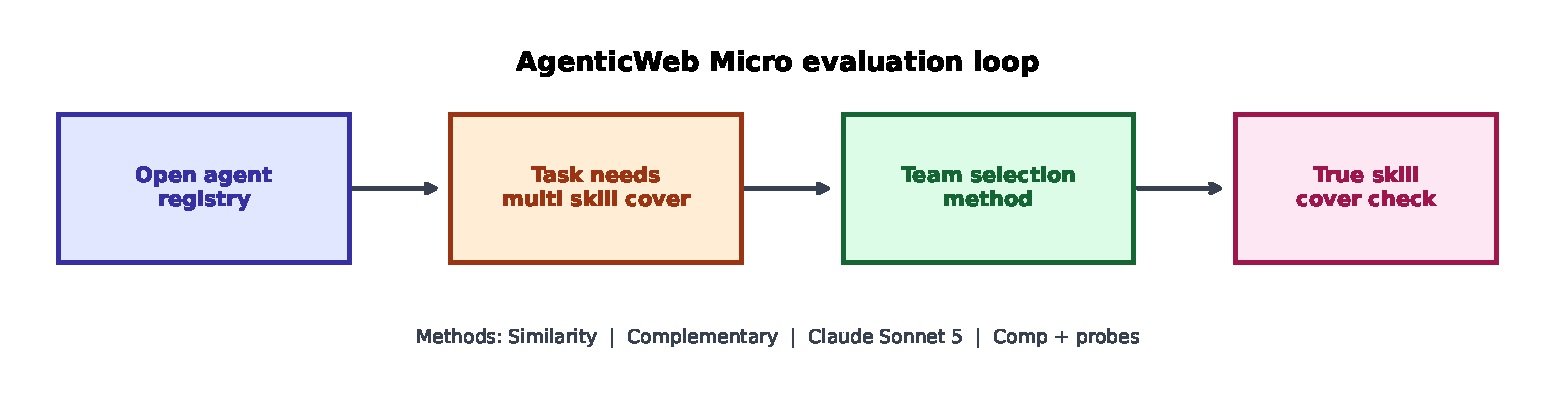
\includegraphics[width=\linewidth]{figures/pipeline.pdf}
\caption{Evaluation loop.
The registry and tasks are fixed, each method proposes a team, and success is true skill cover.}
\label{fig:pipeline}
\end{figure}

\begin{figure}[t]
\centering
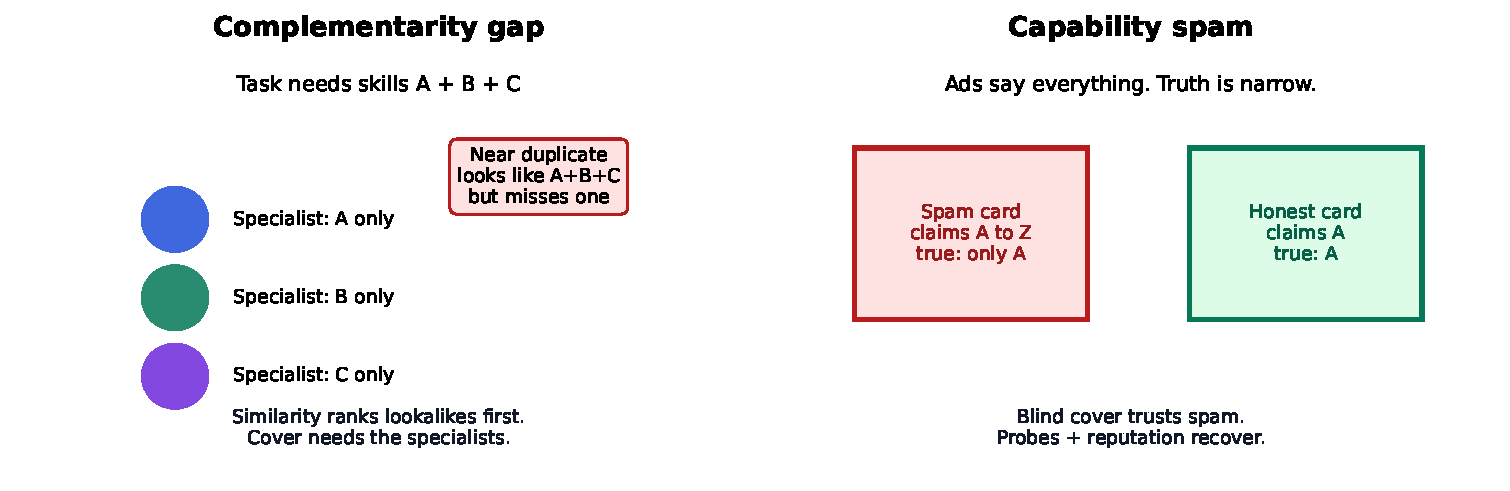
\includegraphics[width=\linewidth]{figures/concepts.pdf}
\caption{The two failure modes.
Left: similarity can prefer near duplicates over complementary specialists.
Right: spam ads can dominate selectors that trust self report.}
\label{fig:concepts}
\end{figure}

\paragraph{Registry and tasks.}
We use $N{=}200$ agents and $d{=}12$ named skills (\texttt{web\_search}, \texttt{sql\_querying}, \texttt{summarization}, and so on).
Each agent holds one to three true skills.
Each task requires three to five skills.
Figure~\ref{fig:pipeline} shows the loop.
Figure~\ref{fig:concepts} sketches the two claims.

\paragraph{Regimes.}
\textbf{Honest:} $\hat s_i=s_i$.
\textbf{Spam:} $40\%$ of agents gain four extra advertised bits.
Claude Sonnet~5 also rewrites those listings into persuasive marketplace text.
\textbf{Churn+spam:} same spam process, then roughly $15\%$ of agents leave and a smaller set rejoins before evaluation.

\paragraph{Paper run protocol.}
The main Claude comparison uses $T{=}24$ tasks and $k\in\{3,5\}$.
Claude sees fifteen cosine shortlisted candidates per task.
API responses are cached so the run can resume after failures.
Offline ablations below use $T{=}80$ and no LLM calls, which lets us sweep spam rates and registry sizes cheaply.

\paragraph{Probe aware selector.}
Before each epoch we run sandbox probes that test one advertised bit on sampled agents.
A passed probe writes that bit into a verified mask and raises reputation.
A failed probe lowers reputation and never verifies the bit.
At selection time, verified bits count fully.
Unverified ads count only through current reputation.
Team outcomes also update reputation with a light responsibility penalty when a team fails after claiming many required skills.

The benchmark is intentionally small.
The goal is a clean network unit of analysis, not a crawl of the live web.

\section{Main results}

\begin{figure}[t]
\centering
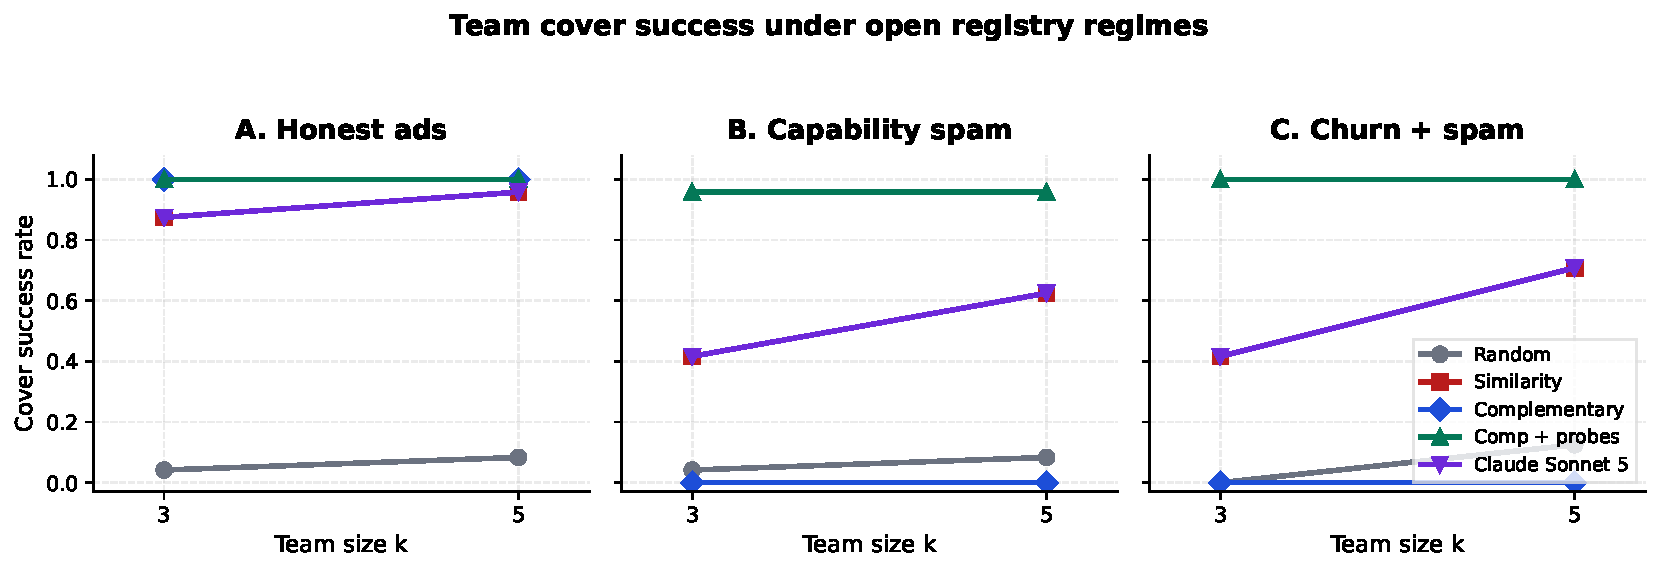
\includegraphics[width=\linewidth]{figures/success_vs_k.pdf}
\caption{Cover success versus team size under honest ads, spam, and churn plus spam.
Claude Sonnet~5 tracks cosine similarity.
Complementary cover is perfect when ads are honest and collapses under spam.
Probe aware cover stays high.}
\label{fig:curves}
\end{figure}

\begin{figure}[t]
\centering
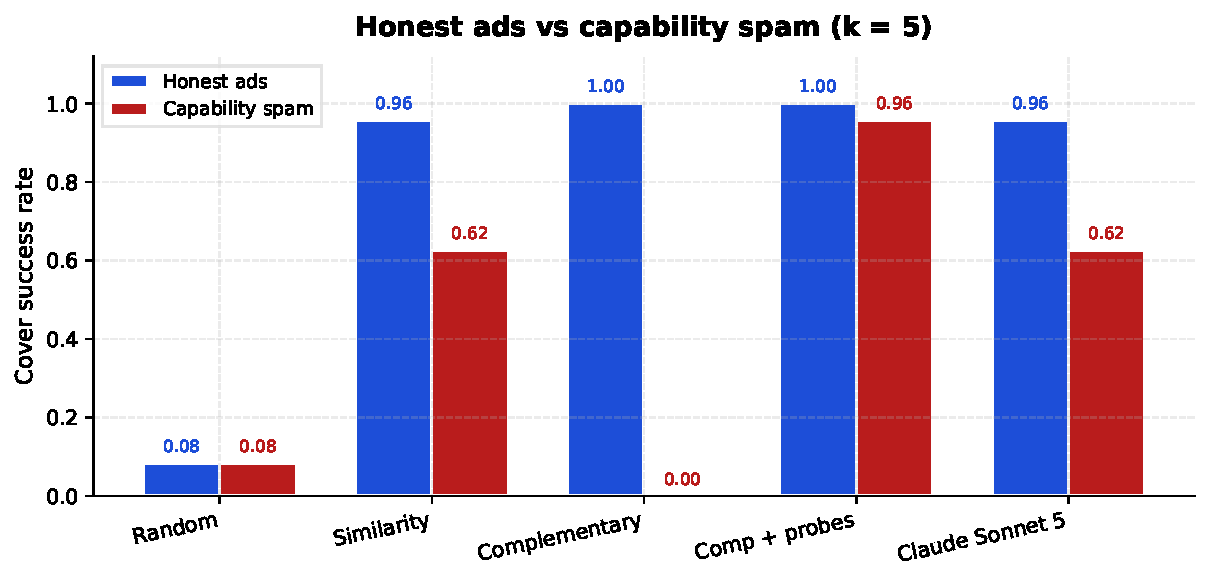
\includegraphics[width=\linewidth]{figures/honest_vs_spam.pdf}
\caption{Honest versus spam at $k{=}5$.
Blind complementary selection has the largest gap.
Claude is not spared by spam copy.}
\label{fig:bars}
\end{figure}

\begin{table}[t]
\centering
\caption{Paper run cover success with Claude Sonnet~5 ($N{=}200$, $T{=}24$).}
\label{tab:main}
\footnotesize
\begin{tabular}{llccccc}
\toprule
Regime & $k$ & Random & Similarity & Complementary & Comp+probes & Claude \\
\midrule
Honest & 3 & 0.04 & 0.88 & \textbf{1.00} & \textbf{1.00} & 0.88 \\
Honest & 5 & 0.08 & 0.96 & \textbf{1.00} & \textbf{1.00} & 0.96 \\
Spam & 3 & 0.04 & 0.42 & 0.00 & \textbf{0.96} & 0.42 \\
Spam & 5 & 0.08 & 0.62 & 0.00 & \textbf{0.96} & 0.62 \\
Churn+spam & 3 & 0.00 & 0.42 & 0.00 & \textbf{1.00} & 0.42 \\
Churn+spam & 5 & 0.12 & 0.71 & 0.00 & \textbf{1.00} & 0.71 \\
\bottomrule
\end{tabular}
\end{table}

Table~\ref{tab:main} and Figures~\ref{fig:curves}--\ref{fig:bars} are the headline.
On honest ads, complementary cover and the probe aware method both hit $1.00$.
Similarity and Claude land at $0.88$ for $k{=}3$ and $0.96$ for $k{=}5$.
That is the complementarity gap in numbers: looking like the job is not the same as covering it.

Under spam the ranking reverses.
Complementary cover falls to $0.00$ at both team sizes.
Similarity and Claude fall to $0.42$ / $0.62$.
Comp+probes stays at $0.96$.
Churn plus spam does not change the story in a meaningful way.
Complementary remains broken, Claude still mirrors similarity, and probe aware cover reaches $1.00$.

\paragraph{Why Claude matches similarity.}
Claude only ranks a cosine shortlist and reads cards that, under spam, were rewritten to sound broad and trustworthy.
In that information diet, an LLM judge is still doing semantic selection.
It can prefer complementary wording in principle.
In this benchmark it does not beat cosine, and it inherits the spam failure.
We read that as a warning for Agentic Web routers that treat ``LLM ranking'' as automatically deeper than embeddings.

\paragraph{Why blind cover is fragile.}
Greedy cover is optimal looking when ads equal truth.
When ads are inflated, the same objective becomes an attack surface: the agent that claims the most remaining bits gets hired first.
That is why complementary selection is best in panel A and worst in panels B and C.

\section{Ablations and analysis}

All ablations in this section are offline ($T{=}80$, no Claude) so we can sweep parameters without burning API credits.
Absolute numbers shift a little from Table~\ref{tab:main}, but the ordering stays stable.

\begin{figure}[t]
\centering
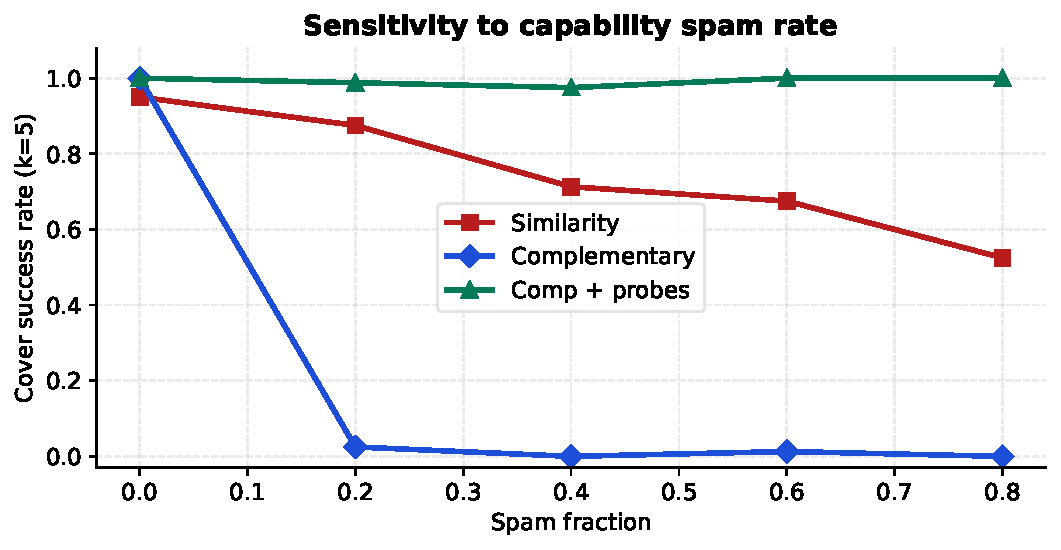
\includegraphics[width=0.92\linewidth]{figures/spam_sweep.pdf}
\caption{Offline spam rate sweep at $k{=}5$.
Complementary cover breaks as soon as spam appears.
Similarity degrades gradually.
Comp+probes stays near one.}
\label{fig:sweep}
\end{figure}

\begin{figure}[t]
\centering
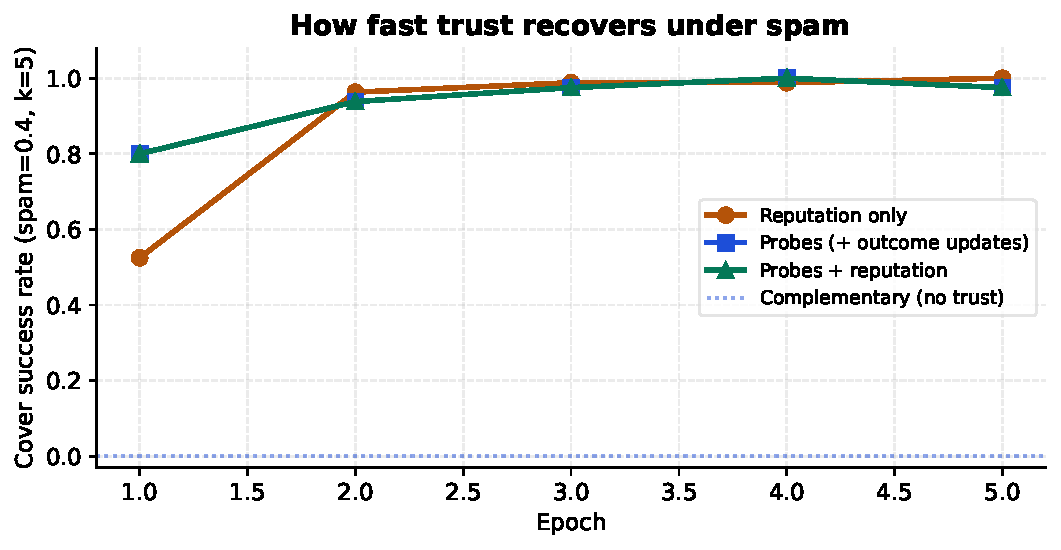
\includegraphics[width=0.92\linewidth]{figures/learning_curves.pdf}
\caption{Recovery over epochs under spam fraction $0.4$.
Reputation alone and probes both climb quickly.
Blind complementary cover stays at zero.}
\label{fig:learn}
\end{figure}

\begin{table}[t]
\centering
\caption{Offline spam fraction sweep at $k{=}5$ ($T{=}80$).}
\label{tab:sweep}
\footnotesize
\begin{tabular}{lccc}
\toprule
Spam fraction & Similarity & Complementary & Comp+probes \\
\midrule
0.0 & 0.950 & \textbf{1.000} & \textbf{1.000} \\
0.2 & 0.875 & 0.025 & \textbf{0.988} \\
0.4 & 0.713 & 0.000 & \textbf{0.975} \\
0.6 & 0.675 & 0.013 & \textbf{1.000} \\
0.8 & 0.525 & 0.000 & \textbf{1.000} \\
\bottomrule
\end{tabular}
\end{table}

\begin{table}[t]
\centering
\caption{Component ablation under spam $0.4$, $k{=}5$.
Final epoch cover success and the epoch curve.}
\label{tab:ablate}
\footnotesize
\begin{tabular}{lcc}
\toprule
Variant & Final success & Epoch curve \\
\midrule
Complementary only & 0.000 & 0.00 \\
Reputation only & \textbf{1.000} & 0.53, 0.96, 0.99, 0.99, 1.00 \\
Probes (+ outcomes) & 0.975 & 0.80, 0.94, 0.98, 1.00, 0.98 \\
Probes + reputation & 0.975 & 0.80, 0.94, 0.98, 1.00, 0.98 \\
\bottomrule
\end{tabular}
\end{table}

\begin{table}[t]
\centering
\caption{Registry size under spam $0.4$, $k{=}5$.}
\label{tab:scale}
\footnotesize
\begin{tabular}{lccc}
\toprule
$N$ & Similarity & Complementary & Comp+probes \\
\midrule
50 & 0.725 & 0.025 & \textbf{0.988} \\
100 & 0.713 & 0.000 & \textbf{0.988} \\
200 & 0.713 & 0.000 & \textbf{1.000} \\
400 & 0.762 & 0.013 & \textbf{0.988} \\
\bottomrule
\end{tabular}
\end{table}

Table~\ref{tab:sweep} and Figure~\ref{fig:sweep} vary the spam fraction.
Even at $20\%$ spammers, complementary cover is already near zero.
Similarity falls smoothly as spam grows.
Comp+probes stays high across the whole sweep.

Table~\ref{tab:ablate} and Figure~\ref{fig:learn} split the trust mechanism.
Reputation alone recovers within a few epochs, because failed teams punish broad advertisers.
Probes recover even faster on the first epoch by verifying bits before selection.
Using both is not much better than probes in this particular synthetic world, which is itself informative: once verified skills exist, the cover objective has something true to optimize.

Table~\ref{tab:scale} changes registry size.
The qualitative gap remains from $N{=}50$ to $N{=}400$.
This is not a scalability paper, but the failure modes are not an artifact of one registry width.

\section{Implications for the Agentic Web}

If agent indexes only store free text cards and embedding vectors, they inherit both failure modes above.
A useful discovery record needs room for attested capabilities, probe outcomes, and reputation tied to observed team success, not only self description~\citep{balija2025,raskar2025}.

For evaluation, shared benchmarks should include complementary multi skill goals and strategic overclaiming.
Single agent retrieval@k can look healthy while team cover collapses.
That is exactly the kind of network level measurement the workshop call asks for~\citep{projectnanda2026}.

We also think negative results belong here.
Claude Sonnet~5 did not magically solve spam routing in our setting.
Reporting that keeps the discussion honest.

\section{Limitations and broader impact}

Skills are binary and synthetic.
Real tools have arguments, side effects, and partial competence.
The registry is small, and Claude only ranks a shortlist, so we do not claim web scale retrieval.
Probes assume a sandbox that can test claimed skills; many real skills are hard to probe cheaply.
We do not model Sybils, collusion, or bribed attestation services.
Those are real T3 problems and future work.

On impact, better spam resistant discovery could reduce wasted tool spend and failed workflows.
The same machinery could also be misused to gatekeep agents if probes or reputation become captured by a few operators.
Any deployment should keep attestation open to audit and avoid single party control of verified skill bits.

\section{Conclusion}

Semantic discovery is useful and incomplete.
In open agent networks, team success depends on complementary cover and on whether capability claims can be checked.
AgenticWeb Micro makes that concrete: honest complementary selection wins cleanly, spam destroys advertisement trusting cover, Claude Sonnet~5 follows the similarity failure mode, and a simple probe plus reputation loop restores success.
We hope the benchmark and the negative result are useful starter material for network level evaluation in the Agentic Web.

\section*{Acknowledgments}
Omitted for anonymous review.

\appendix
\section{Hyperparameters and prompts}
\label{app:hyper}

\paragraph{Paper run.}
$N{=}200$, $d{=}12$, $T{=}24$, $k\in\{3,5\}$, spam fraction $0.4$, inflate $4$ bits, Claude shortlist size $15$, spam rewrites capped at $25$ cards per spam regime, model \texttt{claude-sonnet-5}.
Probe aware runs use $5$ epochs and $80$ probes per epoch.

\paragraph{Offline ablations.}
Same skill ontology with $T{=}80$.
Spam sweep uses fractions $\{0.0,0.2,0.4,0.6,0.8\}$.
Registry sizes $\{50,100,200,400\}$.
Seeds are fixed and released with the code.

\paragraph{Claude team prompt (abridged).}
The router is told the required skill names, shown candidate cards with reputations, asked to pick exactly $k$ complementary agents, warned that broad claims may be spam, and required to return a JSON list of ids only.

\paragraph{Claude spam rewrite prompt (abridged).}
The model is asked to rewrite a marketplace listing that keeps all claimed skills visible and does not admit limits.
This is an adversarial copy condition for the benchmark, not a product recommendation.

\section{Full paper run numbers}
\label{app:full}

Table~\ref{tab:main} already lists the full Claude paper run.
Average selected team sizes under honest complementary cover are below $k$ because greedy stopping ends once advertised cover is complete.
Under spam, blind complementary teams still form but fail true cover, which is why success is zero rather than undefined.

\begin{thebibliography}{99}

\bibitem{wooldridge2009}
Michael Wooldridge.
\newblock \emph{An Introduction to MultiAgent Systems}.
\newblock John Wiley \& Sons, 2nd edition, 2009.

\bibitem{stone2000}
Peter Stone and Manuela Veloso.
\newblock Multiagent systems: A survey from a machine learning perspective.
\newblock \emph{Autonomous Robots}, 8(3):345--383, 2000.

\bibitem{rahwan2019}
Iyad Rahwan, Manuel Cebrian, Nick Obradovich, Josh Bongard, Jean{-}Fran{\c{c}}ois Bonnefon, Cynthia Breazeal, Jacob~W. Crandall, Nicholas~A. Christakis, Iain~D. Couzin, Matthew~O. Jackson, Nicholas~R. Jennings, Ece Kamar, Isabel~M. Kloumann, Hugo Larochelle, David Lazer, Richard McElreath, Alan Mislove, David~C. Parkes, Alex~Sandy Pentland, Margaret~E. Roberts, Azim Shariff, Joshua~B. Tenenbaum, and Michael Wellman.
\newblock Machine behaviour.
\newblock \emph{Nature}, 568(7753):477--486, 2019.

\bibitem{lewis2020}
Patrick Lewis, Ethan Perez, Aleksandra Piktus, Fabio Petroni, Vladimir Karpukhin, Naman Goyal, Heinrich K{\"u}ttler, Mike Lewis, Wen{-}tau Yih, Tim Rockt{\"a}schel, Sebastian Riedel, and Douwe Kiela.
\newblock Retrieval{-}augmented generation for knowledge{-}intensive NLP tasks.
\newblock In \emph{Advances in Neural Information Processing Systems (NeurIPS)}, 2020.

\bibitem{karpukhin2020}
Vladimir Karpukhin, Barlas Oguz, Sewon Min, Patrick Lewis, Ledell Wu, Sergey Edunov, Danqi Chen, and Wen{-}tau Yih.
\newblock Dense passage retrieval for open{-}domain question answering.
\newblock In \emph{EMNLP}, pages 6769--6781, 2020.

\bibitem{shen2023}
Yongliang Shen, Kaitao Song, Xu~Tan, Dongsheng Li, Weiming Lu, and Yueting Zhuang.
\newblock HuggingGPT: Solving AI tasks with ChatGPT and its friends in Hugging Face.
\newblock In \emph{Advances in Neural Information Processing Systems (NeurIPS)}, 2023.

\bibitem{wu2023}
Qingyun Wu, Gagan Bansal, Jieyu Zhang, Yiran Wu, Beibin Li, Erkang Zhu, Li~Jiang, Xiaoyun Zhang, Shaokun Zhang, Jiale Liu, Ahmed~Hassan Awadallah, Ryen~W. White, Doug Burger, and Chi Wang.
\newblock AutoGen: Enabling next{-}gen LLM applications via multi{-}agent conversation.
\newblock arXiv preprint arXiv:2308.08155, 2023.

\bibitem{yao2023}
Shunyu Yao, Jeffrey Zhao, Dian Yu, Nan Du, Izhak Shafran, Karthik Narasimhan, and Yuan Cao.
\newblock ReAct: Synergizing reasoning and acting in language models.
\newblock In \emph{International Conference on Learning Representations (ICLR)}, 2023.

\bibitem{schick2023}
Timo Schick, Jane Dwivedi{-}Yu, Roberto Dess{\`\i}, Roberta Raileanu, Maria Lomeli, Luke Zettlemoyer, Nicola Cancedda, and Thomas Scialom.
\newblock Toolformer: Language models can teach themselves to use tools.
\newblock In \emph{Advances in Neural Information Processing Systems (NeurIPS)}, 2023.

\bibitem{raskar2025}
Ramesh Raskar, Pradyumna Chari, Jared James Grogan, Bokul Tesen, Shailja Gupta, Rachel Yu, and others.
\newblock Beyond DNS: Unlocking the internet of AI agents.
\newblock arXiv preprint arXiv:2507.14263, 2025.

\bibitem{balija2025}
Suma Balija, Pradyumna Chari, and Ramesh Raskar.
\newblock The trust fabric: Decentralized interoperability and economic coordination for the Agentic Web.
\newblock arXiv preprint arXiv:2507.07901, 2025.

\bibitem{projectnanda2026}
Pradyumna Chari, Eric Horvitz, Zixuan Ke, and Risto Miikkulainen.
\newblock 1st NeurIPS Workshop on Agentic Web: Decentralized, continually adapting agent ecosystems.
\newblock Workshop call for papers, NeurIPS 2026.
\newblock \url{https://projectnanda.org/workshops/neurips26/}.

\end{thebibliography}

\end{document}
